\chapter{Implementation Overview}
\label{ch:developers_guide}
\label{ch:programmers_guide}

When creating our application, we kept in mind to make it as easy as possible for user to use. We therefore selected a web-based front-end, with which users come in contact daily. From the user point of view, it does not require installation of any application and it can be used from almost any platform.

Creating simple, shareable environment from the user perspective gives us opportunity of collecting more annotated data by the users. Comparing to the classical applications, which need to be installed and run, using a web-based application is enough to run it on the server by researcher and share the links with the respondents. This way it may be easier to reach bigger audience.

We decided to use Python for our back-end as it has big machine learning community with ever growing possibilities of open-source projects. As the results of this, we decided to use Django easily scalable Python web-framework.

Since our implementation covers a wide range of tasks -- from a web-based front-end to library able to work with deep learning models. We do not include an exhaustive enumeration of the specific classes/functions in this chapter. Rather we provide an overview of the individual parts of the application. We start with the separation of the application into three layers, as displayed in figure \ref{fig:implementation_overview}.

This figure represents the individual layers of our solution and provides a summary of the technologies used in the layers. Our application consists of two main Python modules: \verb+diplomova_praca+ and \verb+diplomova_praca_lib+. In the figure, the front-end and backend belong to the first one, and the library represents module \verb+diplomova_praca_lib+.

We shortly describe each of the parts, as displayed in the figure.

\section{Front-end}

Our front-end consists of several Django templates (a way to create HTML files dynamically), with the corresponding styling. We then use jQuery to provide a user with an interactive environment in the application.  The part of displaying the menu and the results are shared between both modules -- face and spatial. The interactive content -- canvas for the spatial and the grid for faces -- is dynamically added based on the currently selected module.

\subsubsection*{Design}
For a unified look, we follow the Material Design guidelines. We use some of the components from Material Design Lite. To complement the overall design, we also use the Material Design Icons.

We use the Material Design components with our own elements using the Cascading Style Sheets. We use Syntactically Awesome Style Sheets (commonly known as SCSS) to reduce the amount of code. One of the advantages of SCSS compared to CSS is the support of variables and nesting. We use this, for example, when setting the colors for the whole application. This way, we can provide users with a unified color scheme, while the colors can be easily adjusted for a different color scheme.

\subsubsection*{Interaction}

To provide smooth user experience, without any unnecessary during the search, we use JavaScript. For some actions, like dragging, resizing we utilize functionalities from jQuery\footnote{\url{https://jquery.com/}}. 

To avoid reloadings we update the content using JavaScript and obtain the data via asynchronous communication with our Django backend. One of the advantages of this approach is that the user can continue to experiment with the collage while the system is retrieving the results.

We do the communication with the Django as asynchronous HTTP POST requests. We encode the data as JSON, or directly as a string, if possible. The data are of different types; for example, in the spatial module, we need to send all images with their relative position. In the case of the face module, we include the Tree View, i.e., the current level and position in the layer.

\section{Back-end}

The goal of our backend is to process the HTTP requests from front-end and transform them into Python objects. This way, we can directly query our library by calling the functions by passing the Python objects. The backend also initializes the datasets in the library. Additional functionality of the backend is the choice of the target image out of available images. Secondary functionalities include logging submitted collages and additional data into the database.

\section{Library}

In the library, we implement all approaches mentioned in this thesis. The library includes all the feature extraction methods, image handling, training, plots generation, and more.

Since the content of the library is broad, we could separate it further into four main blocks: 
\begin{itemize}
    \item Annotation and Preprocessing -- scripts used for extraction of the features from custom dataset
    \item \verb+face_features/+ -- face module, which is responsible for creating the multilevel structure (\verb+TreeView+). It also contains models for extraction of faces and the feature extraction.
    \item \verb+position_similarity/+ -- spatial module, which also includes used models and the feature extraction techniques (as regions or antepenultime approach). The entry point for any request is \verb+positional_request()+ in \verb+position_similarity_request.py+. We use this entry point for our experiments.
    \item Additional scripts (\verb+helpers/+) -- this includes all scripts to run and evaluate the experiments.. These are not necessary for the application itself, but useful while investigating the approaches.
\end{itemize}

\subsubsection*{Attribution}

At last, we would like to express our grattitude to the authors of all used technologies provided by an open-source community. Additionally to the projects mentioned in the text we would like to thank also the authors of crucial libraries such as Scikit-learn \citep{pedregosa2011scikit} and NumPy \citep{van2011numpy}.

\begin{figure}
    \centering
    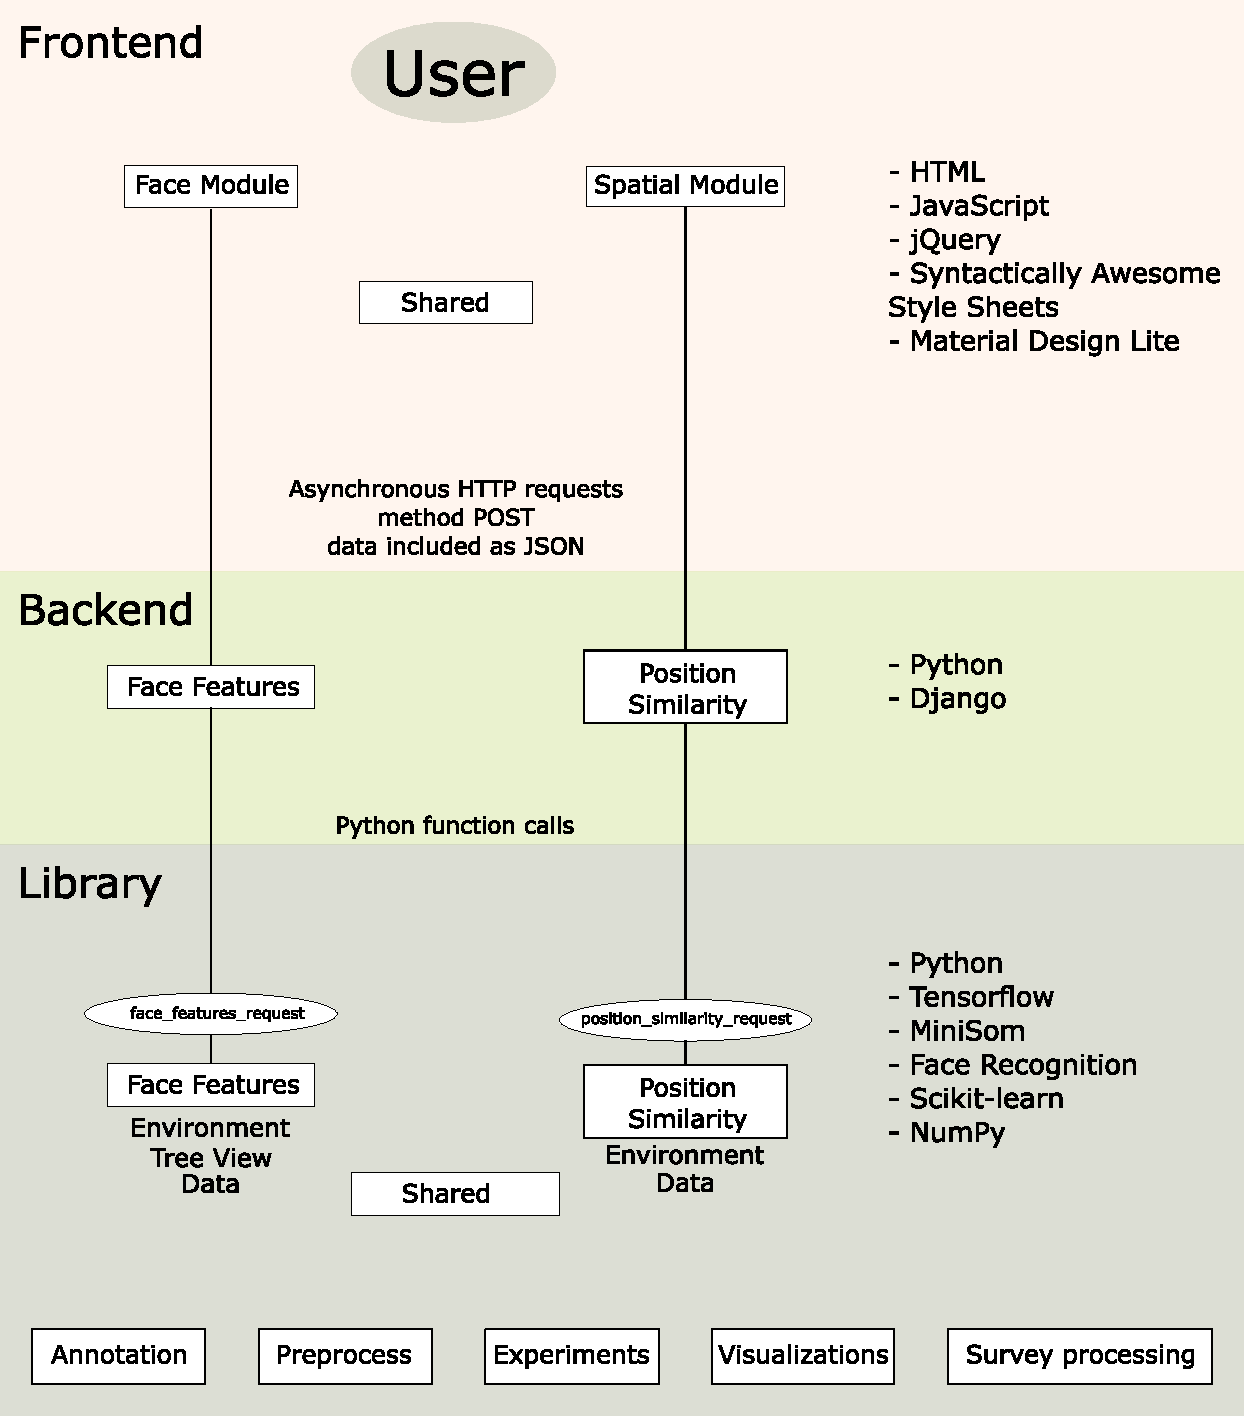
\includegraphics[width=0.95\linewidth]{graphs/implementation_overview.pdf}
    \caption{Overview of the implementation}
    \label{fig:implementation_overview}
\end{figure}